\documentclass[twoside]{article}

% Packages required by doxygen
\usepackage{fixltx2e}
\usepackage{calc}
\usepackage{doxygen}
\usepackage{graphicx}
\usepackage[utf8]{inputenc}
\usepackage{makeidx}
\usepackage{multicol}
\usepackage{multirow}
\PassOptionsToPackage{warn}{textcomp}
\usepackage{textcomp}
\usepackage[nointegrals]{wasysym}
\usepackage[table]{xcolor}

% NLS support packages
\usepackage[french]{babel}

% Font selection
\usepackage[T1]{fontenc}
\usepackage{mathptmx}
\usepackage[scaled=.90]{helvet}
\usepackage{courier}
\usepackage{amssymb}
\usepackage{sectsty}
\renewcommand{\familydefault}{\sfdefault}
\allsectionsfont{%
  \fontseries{bc}\selectfont%
  \color{darkgray}%
}
\renewcommand{\DoxyLabelFont}{%
  \fontseries{bc}\selectfont%
  \color{darkgray}%
}
\newcommand{\+}{\discretionary{\mbox{\scriptsize$\hookleftarrow$}}{}{}}

% Page & text layout
\usepackage{geometry}
\geometry{%
  a4paper,%
  top=2.5cm,%
  bottom=2.5cm,%
  left=2.5cm,%
  right=2.5cm%
}
\tolerance=750
\hfuzz=15pt
\hbadness=750
\setlength{\emergencystretch}{15pt}
\setlength{\parindent}{0cm}
\setlength{\parskip}{0.2cm}
\makeatletter
\renewcommand{\paragraph}{%
  \@startsection{paragraph}{4}{0ex}{-1.0ex}{1.0ex}{%
    \normalfont\normalsize\bfseries\SS@parafont%
  }%
}
\renewcommand{\subparagraph}{%
  \@startsection{subparagraph}{5}{0ex}{-1.0ex}{1.0ex}{%
    \normalfont\normalsize\bfseries\SS@subparafont%
  }%
}
\makeatother

% Headers & footers
\usepackage{fancyhdr}
\pagestyle{fancyplain}
\fancyhead[LE]{\fancyplain{}{\bfseries\thepage}}
\fancyhead[CE]{\fancyplain{}{}}
\fancyhead[RE]{\fancyplain{}{\bfseries\leftmark}}
\fancyhead[LO]{\fancyplain{}{\bfseries\rightmark}}
\fancyhead[CO]{\fancyplain{}{}}
\fancyhead[RO]{\fancyplain{}{\bfseries\thepage}}
\fancyfoot[LE]{\fancyplain{}{}}
\fancyfoot[CE]{\fancyplain{}{}}
\fancyfoot[RE]{\fancyplain{}{\bfseries\scriptsize Généré le Vendredi 25 Septembre 2015 11\+:04\+:03 pour libjournal par Doxygen }}
\fancyfoot[LO]{\fancyplain{}{\bfseries\scriptsize Généré le Vendredi 25 Septembre 2015 11\+:04\+:03 pour libjournal par Doxygen }}
\fancyfoot[CO]{\fancyplain{}{}}
\fancyfoot[RO]{\fancyplain{}{}}
\renewcommand{\footrulewidth}{0.4pt}
\renewcommand{\sectionmark}[1]{%
  \markright{\thesection\ #1}%
}

% Indices & bibliography
\usepackage{natbib}
\usepackage[titles]{tocloft}
\setcounter{tocdepth}{3}
\setcounter{secnumdepth}{5}
\makeindex

% Hyperlinks (required, but should be loaded last)
\usepackage{ifpdf}
\ifpdf
  \usepackage[pdftex,pagebackref=true]{hyperref}
\else
  \usepackage[ps2pdf,pagebackref=true]{hyperref}
\fi
\hypersetup{%
  colorlinks=true,%
  linkcolor=blue,%
  citecolor=blue,%
  unicode%
}

% Custom commands
\newcommand{\clearemptydoublepage}{%
  \newpage{\pagestyle{empty}\cleardoublepage}%
}


%===== C O N T E N T S =====

\begin{document}

% Titlepage & ToC
\hypersetup{pageanchor=false,
             bookmarks=true,
             bookmarksnumbered=true,
             pdfencoding=unicode
            }
\pagenumbering{roman}
\begin{titlepage}
\vspace*{7cm}
\begin{center}%
{\Large libjournal \\[1ex]\large 1.\+1.\+57 }\\
\vspace*{1cm}
{\large Généré par Doxygen 1.8.8}\\
\vspace*{0.5cm}
{\small Vendredi 25 Septembre 2015 11:04:03}\\
\end{center}
\end{titlepage}
\tableofcontents
\pagenumbering{arabic}
\hypersetup{pageanchor=true}

%--- Begin generated contents ---
\section{Index des fichiers}
\subsection{Liste des fichiers}
Liste de tous les fichiers avec une brève description \+:\begin{DoxyCompactList}
\item\contentsline{section}{lib/\hyperlink{journal_8h}{journal.\+h} }{\pageref{journal_8h}}{}
\end{DoxyCompactList}

\section{Documentation des fichiers}
\hypertarget{journal_8h}{\subsection{Référence du fichier lib/journal.h}
\label{journal_8h}\index{lib/journal.\+h@{lib/journal.\+h}}
}
{\ttfamily \#include $<$stdarg.\+h$>$}\\*
{\ttfamily \#include $<$stdio.\+h$>$}\\*
{\ttfamily \#include $<$time.\+h$>$}\\*
Graphe des dépendances par inclusion de journal.\+h\+:
\nopagebreak
\begin{figure}[H]
\begin{center}
\leavevmode
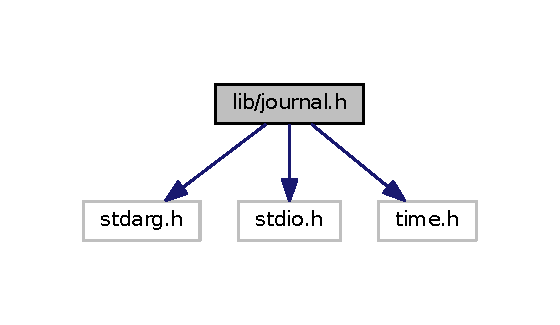
\includegraphics[width=269pt]{journal_8h__incl}
\end{center}
\end{figure}
\subsubsection*{Macros}
\begin{DoxyCompactItemize}
\item 
\#define \hyperlink{journal_8h_a0c68e1a9decbf8ce8463bd7af26e0690}{J\+O\+U\+R\+N\+A\+L}(niveau, args...)~\hyperlink{journal_8h_a75d3b5d4af49473d5318043f90effb0e}{ecrire\+\_\+entree\+\_\+journal}(niveau, \+\_\+\+\_\+\+F\+I\+L\+E\+\_\+\+\_\+, \+\_\+\+\_\+\+L\+I\+N\+E\+\_\+\+\_\+, args)
\end{DoxyCompactItemize}
\subsubsection*{Énumérations}
\begin{DoxyCompactItemize}
\item 
enum \hyperlink{journal_8h_ae325737a61040fd711e0b223515d9939}{niveau\+\_\+t} \{ \\*
\hyperlink{journal_8h_ae325737a61040fd711e0b223515d9939ac157bdf0b85a40d2619cbc8bc1ae5fe2}{N\+O\+N\+E} = 0, 
\hyperlink{journal_8h_ae325737a61040fd711e0b223515d9939a2fd6f336d08340583bd620a7f5694c90}{E\+R\+R\+O\+R} = 1, 
\hyperlink{journal_8h_ae325737a61040fd711e0b223515d9939a984de77c680eaff141ec910e25568a81}{W\+A\+R\+N\+I\+N\+G} = 2, 
\hyperlink{journal_8h_ae325737a61040fd711e0b223515d9939a748005382152808a72b1a9177d9dc806}{I\+N\+F\+O} = 3, 
\\*
\hyperlink{journal_8h_ae325737a61040fd711e0b223515d9939a0593585da9181e972974c1274d8f2b4f}{D\+E\+B\+U\+G} = 4
 \}
\end{DoxyCompactItemize}
\subsubsection*{Fonctions}
\begin{DoxyCompactItemize}
\item 
int \hyperlink{journal_8h_ac9d615c5f58ac546ad841232698ff2ba}{ouvrir\+\_\+journal} (\hyperlink{journal_8h_ae325737a61040fd711e0b223515d9939}{niveau\+\_\+t} niveau, char $\ast$nom\+\_\+fichier, F\+I\+L\+E $\ast$fichier, int ajouter)
\item 
void \hyperlink{journal_8h_a5ba61dfe113b8ba28d0196d7b3f914c6}{fermer\+\_\+journal} (void)
\item 
void \hyperlink{journal_8h_a75d3b5d4af49473d5318043f90effb0e}{ecrire\+\_\+entree\+\_\+journal} (\hyperlink{journal_8h_ae325737a61040fd711e0b223515d9939}{niveau\+\_\+t} niveau, char $\ast$fichier, int ligne, char $\ast$format,...)
\end{DoxyCompactItemize}
\subsubsection*{Variables}
\begin{DoxyCompactItemize}
\item 
static char $\ast$ \hyperlink{journal_8h_ae64d64f064c50b63e815971be0e2e4bf}{niveau\+\_\+vers\+\_\+chaine} \mbox{[}$\,$\mbox{]}
\end{DoxyCompactItemize}


\subsubsection{Documentation des macros}
\hypertarget{journal_8h_a0c68e1a9decbf8ce8463bd7af26e0690}{\index{journal.\+h@{journal.\+h}!J\+O\+U\+R\+N\+A\+L@{J\+O\+U\+R\+N\+A\+L}}
\index{J\+O\+U\+R\+N\+A\+L@{J\+O\+U\+R\+N\+A\+L}!journal.\+h@{journal.\+h}}
\paragraph[{J\+O\+U\+R\+N\+A\+L}]{\setlength{\rightskip}{0pt plus 5cm}\#define J\+O\+U\+R\+N\+A\+L(
\begin{DoxyParamCaption}
\item[{}]{niveau, }
\item[{}]{args...}
\end{DoxyParamCaption}
)~{\bf ecrire\+\_\+entree\+\_\+journal}(niveau, \+\_\+\+\_\+\+F\+I\+L\+E\+\_\+\+\_\+, \+\_\+\+\_\+\+L\+I\+N\+E\+\_\+\+\_\+, args)}}\label{journal_8h_a0c68e1a9decbf8ce8463bd7af26e0690}
M\+A\+C\+R\+O permettant de faciliter l'ajout d'une entrée au journal.

Cette M\+A\+C\+R\+O fournie une interface simplifiée à \hyperlink{journal_8h_a75d3b5d4af49473d5318043f90effb0e}{ecrire\+\_\+entree\+\_\+journal()} en passant les définitions {\ttfamily \+\_\+\+\_\+\+F\+I\+L\+E\+\_\+\+\_\+} et {\ttfamily \+\_\+\+\_\+\+L\+I\+N\+E\+\_\+\+\_\+} correspondant toutes deux au {\bfseries nom du fichier} appelant la M\+A\+C\+R\+O et le {\bfseries numéro de ligne} d'appel à la M\+A\+C\+R\+O, respectivement.

{\bfseries Exemple \+:} 
\begin{DoxyCode}
\textcolor{keywordflow}{if}(\hyperlink{journal_8h_ac9d615c5f58ac546ad841232698ff2ba}{ouvrir\_journal}(\hyperlink{journal_8h_ae325737a61040fd711e0b223515d9939a2fd6f336d08340583bd620a7f5694c90}{ERROR}, \textcolor{stringliteral}{"mon\_journal.log"}, NULL, 0) != 0)
\{
   \textcolor{keywordflow}{return} 1;
\}
\textcolor{keywordflow}{else}\{
   \textcolor{keywordtype}{char}* message = \textcolor{stringliteral}{"Bonjour le monde !"};
   \hyperlink{journal_8h_a0c68e1a9decbf8ce8463bd7af26e0690}{JOURNAL}(\hyperlink{journal_8h_ae325737a61040fd711e0b223515d9939a0593585da9181e972974c1274d8f2b4f}{DEBUG}, \textcolor{stringliteral}{"Le message de DEBUG est : %s"}, message);
\}
\end{DoxyCode}



\begin{DoxyParams}{Paramètres}
{\em niveau} & Le niveau de criticité de l'entrée. \\
\hline
{\em args} & La chaîne de caractères spécifiant le message à journaliser (accompagnée des variables si nécessaire).\\
\hline
\end{DoxyParams}
\begin{DoxySeeAlso}{Voir également}
\hyperlink{journal_8h_a75d3b5d4af49473d5318043f90effb0e}{ecrire\+\_\+entree\+\_\+journal()} 
\end{DoxySeeAlso}


\subsubsection{Documentation du type de l'énumération}
\hypertarget{journal_8h_ae325737a61040fd711e0b223515d9939}{\index{journal.\+h@{journal.\+h}!niveau\+\_\+t@{niveau\+\_\+t}}
\index{niveau\+\_\+t@{niveau\+\_\+t}!journal.\+h@{journal.\+h}}
\paragraph[{niveau\+\_\+t}]{\setlength{\rightskip}{0pt plus 5cm}enum {\bf niveau\+\_\+t}}}\label{journal_8h_ae325737a61040fd711e0b223515d9939}
Énumération des différents niveaux de criticité de journalisation.

Chaque énumération peut être convertie en chaîne de caractère grâce à la structure de données niveau\+\_\+vers\+\_\+chaine\mbox{[}\mbox{]}.

\begin{DoxySeeAlso}{Voir également}
\hyperlink{journal_8h_ae64d64f064c50b63e815971be0e2e4bf}{niveau\+\_\+vers\+\_\+chaine}\mbox{[}\mbox{]} 
\end{DoxySeeAlso}
\begin{Desc}
\item[Valeurs énumérées]\par
\begin{description}
\index{N\+O\+N\+E@{N\+O\+N\+E}!journal.\+h@{journal.\+h}}\index{journal.\+h@{journal.\+h}!N\+O\+N\+E@{N\+O\+N\+E}}\item[{\em 
\hypertarget{journal_8h_ae325737a61040fd711e0b223515d9939ac157bdf0b85a40d2619cbc8bc1ae5fe2}{N\+O\+N\+E}\label{journal_8h_ae325737a61040fd711e0b223515d9939ac157bdf0b85a40d2619cbc8bc1ae5fe2}
}]\index{E\+R\+R\+O\+R@{E\+R\+R\+O\+R}!journal.\+h@{journal.\+h}}\index{journal.\+h@{journal.\+h}!E\+R\+R\+O\+R@{E\+R\+R\+O\+R}}\item[{\em 
\hypertarget{journal_8h_ae325737a61040fd711e0b223515d9939a2fd6f336d08340583bd620a7f5694c90}{E\+R\+R\+O\+R}\label{journal_8h_ae325737a61040fd711e0b223515d9939a2fd6f336d08340583bd620a7f5694c90}
}]\index{W\+A\+R\+N\+I\+N\+G@{W\+A\+R\+N\+I\+N\+G}!journal.\+h@{journal.\+h}}\index{journal.\+h@{journal.\+h}!W\+A\+R\+N\+I\+N\+G@{W\+A\+R\+N\+I\+N\+G}}\item[{\em 
\hypertarget{journal_8h_ae325737a61040fd711e0b223515d9939a984de77c680eaff141ec910e25568a81}{W\+A\+R\+N\+I\+N\+G}\label{journal_8h_ae325737a61040fd711e0b223515d9939a984de77c680eaff141ec910e25568a81}
}]\index{I\+N\+F\+O@{I\+N\+F\+O}!journal.\+h@{journal.\+h}}\index{journal.\+h@{journal.\+h}!I\+N\+F\+O@{I\+N\+F\+O}}\item[{\em 
\hypertarget{journal_8h_ae325737a61040fd711e0b223515d9939a748005382152808a72b1a9177d9dc806}{I\+N\+F\+O}\label{journal_8h_ae325737a61040fd711e0b223515d9939a748005382152808a72b1a9177d9dc806}
}]\index{D\+E\+B\+U\+G@{D\+E\+B\+U\+G}!journal.\+h@{journal.\+h}}\index{journal.\+h@{journal.\+h}!D\+E\+B\+U\+G@{D\+E\+B\+U\+G}}\item[{\em 
\hypertarget{journal_8h_ae325737a61040fd711e0b223515d9939a0593585da9181e972974c1274d8f2b4f}{D\+E\+B\+U\+G}\label{journal_8h_ae325737a61040fd711e0b223515d9939a0593585da9181e972974c1274d8f2b4f}
}]\end{description}
\end{Desc}

\begin{DoxyCode}
15              \{
16     \hyperlink{journal_8h_ae325737a61040fd711e0b223515d9939ac157bdf0b85a40d2619cbc8bc1ae5fe2}{NONE} = 0,
17     \hyperlink{journal_8h_ae325737a61040fd711e0b223515d9939a2fd6f336d08340583bd620a7f5694c90}{ERROR} = 1,
18     \hyperlink{journal_8h_ae325737a61040fd711e0b223515d9939a984de77c680eaff141ec910e25568a81}{WARNING} = 2,
19     \hyperlink{journal_8h_ae325737a61040fd711e0b223515d9939a748005382152808a72b1a9177d9dc806}{INFO} = 3,
20     \hyperlink{journal_8h_ae325737a61040fd711e0b223515d9939a0593585da9181e972974c1274d8f2b4f}{DEBUG} = 4,
21 \} \hyperlink{journal_8h_ae325737a61040fd711e0b223515d9939}{niveau\_t};
\end{DoxyCode}


\subsubsection{Documentation des fonctions}
\hypertarget{journal_8h_a75d3b5d4af49473d5318043f90effb0e}{\index{journal.\+h@{journal.\+h}!ecrire\+\_\+entree\+\_\+journal@{ecrire\+\_\+entree\+\_\+journal}}
\index{ecrire\+\_\+entree\+\_\+journal@{ecrire\+\_\+entree\+\_\+journal}!journal.\+h@{journal.\+h}}
\paragraph[{ecrire\+\_\+entree\+\_\+journal}]{\setlength{\rightskip}{0pt plus 5cm}void ecrire\+\_\+entree\+\_\+journal (
\begin{DoxyParamCaption}
\item[{{\bf niveau\+\_\+t}}]{niveau, }
\item[{char $\ast$}]{fichier, }
\item[{int}]{ligne, }
\item[{char $\ast$}]{format, }
\item[{}]{...}
\end{DoxyParamCaption}
)}}\label{journal_8h_a75d3b5d4af49473d5318043f90effb0e}
Écrit une entrée dans le fichier de journalisation.

Ne peut être appellé S\+I E\+T S\+E\+U\+L\+E\+M\+E\+N\+T S\+I ouvrir\+\_\+journal a été appelé et n'a pas retourné d'erreur.

{\bfseries Exemple \+:} 
\begin{DoxyCode}
\textcolor{keywordtype}{char}* message = \textcolor{stringliteral}{"Bonjour le monde !"};
\hyperlink{journal_8h_a75d3b5d4af49473d5318043f90effb0e}{ecrire\_entree\_journal}(\hyperlink{journal_8h_ae325737a61040fd711e0b223515d9939a0593585da9181e972974c1274d8f2b4f}{DEBUG}, \_\_FILE\_\_, \_\_LINE\_\_, \textcolor{stringliteral}{"Le message de DEBUG est : %s"}, 
      message);
\end{DoxyCode}



\begin{DoxyParams}{Paramètres}
{\em niveau} & Le niveau de criticité de l'entrée à journaliser \\
\hline
{\em fichier} & Une chaîne décrivant le fichier réalisant l'entrée. {\ttfamily \+\_\+\+\_\+\+F\+I\+L\+E\+\_\+\+\_\+} est sans nul doute ce que vous préféreriez saisir. \\
\hline
{\em ligne} & Un nombre décrivant le numéro de la ligne réalisant l'entrée. {\ttfamily \+\_\+\+\_\+\+L\+I\+N\+E\+\_\+\+\_\+} est sans nul doute ce que vous préféreriez saisir. \\
\hline
{\em format} & La chaîne de caractères spécifiant le message à journaliser formatée comme une 'printf format string'.\\
\hline
\end{DoxyParams}
\begin{DoxySeeAlso}{Voir également}
\hyperlink{journal_8h_a0c68e1a9decbf8ce8463bd7af26e0690}{J\+O\+U\+R\+N\+A\+L} 
\end{DoxySeeAlso}
\hypertarget{journal_8h_a5ba61dfe113b8ba28d0196d7b3f914c6}{\index{journal.\+h@{journal.\+h}!fermer\+\_\+journal@{fermer\+\_\+journal}}
\index{fermer\+\_\+journal@{fermer\+\_\+journal}!journal.\+h@{journal.\+h}}
\paragraph[{fermer\+\_\+journal}]{\setlength{\rightskip}{0pt plus 5cm}void fermer\+\_\+journal (
\begin{DoxyParamCaption}
\item[{void}]{}
\end{DoxyParamCaption}
)}}\label{journal_8h_a5ba61dfe113b8ba28d0196d7b3f914c6}
Termine l'utilisation possible de la journalisation.

Clos le fichier de journalisation et empêche tout ajout d'une nouvelle entrée au journal.

{\bfseries Exemple \+:} 
\begin{DoxyCode}
\textcolor{keywordflow}{if}(\hyperlink{journal_8h_ac9d615c5f58ac546ad841232698ff2ba}{ouvrir\_journal}(\hyperlink{journal_8h_ae325737a61040fd711e0b223515d9939a2fd6f336d08340583bd620a7f5694c90}{ERROR}, \textcolor{stringliteral}{"mon\_journal.log"}, NULL, 0) != 0)
\{
   \textcolor{keywordflow}{return} 1;
\}
\textcolor{keywordflow}{else}\{
   \textcolor{comment}{// Faire quelque chose}
   \textcolor{comment}{// ...}
   \hyperlink{journal_8h_a5ba61dfe113b8ba28d0196d7b3f914c6}{fermer\_journal}();
\}
\end{DoxyCode}


\begin{DoxySeeAlso}{Voir également}
\hyperlink{journal_8h_ac9d615c5f58ac546ad841232698ff2ba}{ouvrir\+\_\+journal()} 
\end{DoxySeeAlso}
\hypertarget{journal_8h_ac9d615c5f58ac546ad841232698ff2ba}{\index{journal.\+h@{journal.\+h}!ouvrir\+\_\+journal@{ouvrir\+\_\+journal}}
\index{ouvrir\+\_\+journal@{ouvrir\+\_\+journal}!journal.\+h@{journal.\+h}}
\paragraph[{ouvrir\+\_\+journal}]{\setlength{\rightskip}{0pt plus 5cm}int ouvrir\+\_\+journal (
\begin{DoxyParamCaption}
\item[{{\bf niveau\+\_\+t}}]{niveau, }
\item[{char $\ast$}]{nom\+\_\+fichier, }
\item[{F\+I\+L\+E $\ast$}]{fichier, }
\item[{int}]{ajouter}
\end{DoxyParamCaption}
)}}\label{journal_8h_ac9d615c5f58ac546ad841232698ff2ba}
Initialise la journalisation.

{\bfseries Exemple \+:} 
\begin{DoxyCode}
\textcolor{keywordtype}{int} resultat;
resultat = \hyperlink{journal_8h_ac9d615c5f58ac546ad841232698ff2ba}{ouvrir\_journal}(\hyperlink{journal_8h_ae325737a61040fd711e0b223515d9939a2fd6f336d08340583bd620a7f5694c90}{ERROR}, \textcolor{stringliteral}{"mon\_journal.log"}, NULL, 0);
\end{DoxyCode}


ou bien


\begin{DoxyCode}
\textcolor{keywordtype}{int} resultat;
FILE* fichier\_journal\_perso;
fichier\_journal\_perso = fopen(\textcolor{stringliteral}{"mon\_journal.log"}, \textcolor{stringliteral}{"w"});
resultat = \hyperlink{journal_8h_ac9d615c5f58ac546ad841232698ff2ba}{ouvrir\_journal}(\hyperlink{journal_8h_ae325737a61040fd711e0b223515d9939a2fd6f336d08340583bd620a7f5694c90}{ERROR}, NULL, fichier\_journal\_perso, 0);
\end{DoxyCode}
 Ouvrira, par écrasement, le fichier nommé {\ttfamily mon\+\_\+journal.\+log} pour y écrire tout événement de criticité inférieur ou égale à {\ttfamily E\+R\+R\+O\+R} .


\begin{DoxyParams}{Paramètres}
{\em niveau} & Tout futur appel à \hyperlink{journal_8h_a75d3b5d4af49473d5318043f90effb0e}{ecrire\+\_\+entree\+\_\+journal()} ne journalisera qu'à un niveau inférieur ou égal à ce niveau de criticité. \\
\hline
{\em nom\+\_\+fichier} & La chaîne de caractères définissant le chemin du fichier de journalisation (si N\+U\+L\+L, alors fichier doit être valorisé). \\
\hline
{\em fichier} & Pointeur sur F\+I\+L\+E d'un fichier déjà déclaré (si N\+U\+L\+L, alors nom\+\_\+fichier doit être valorisé). \\
\hline
{\em ajouter} & Mode ajout au fichier si différent de 0, mode écrasé si égal à 0.\\
\hline
\end{DoxyParams}
\begin{DoxyReturn}{Renvoie}
0 si tout va bien, -\/1 sinon
\end{DoxyReturn}
\begin{DoxySeeAlso}{Voir également}
\hyperlink{journal_8h_a75d3b5d4af49473d5318043f90effb0e}{ecrire\+\_\+entree\+\_\+journal} 
\end{DoxySeeAlso}


\subsubsection{Documentation des variables}
\hypertarget{journal_8h_ae64d64f064c50b63e815971be0e2e4bf}{\index{journal.\+h@{journal.\+h}!niveau\+\_\+vers\+\_\+chaine@{niveau\+\_\+vers\+\_\+chaine}}
\index{niveau\+\_\+vers\+\_\+chaine@{niveau\+\_\+vers\+\_\+chaine}!journal.\+h@{journal.\+h}}
\paragraph[{niveau\+\_\+vers\+\_\+chaine}]{\setlength{\rightskip}{0pt plus 5cm}char$\ast$ niveau\+\_\+vers\+\_\+chaine\mbox{[}$\,$\mbox{]}\hspace{0.3cm}{\ttfamily [static]}}}\label{journal_8h_ae64d64f064c50b63e815971be0e2e4bf}
{\bfseries Valeur initiale \+:}
\begin{DoxyCode}
= \{
    NULL,
    \textcolor{stringliteral}{"ERROR"},
    \textcolor{stringliteral}{"WARNING"},
    \textcolor{stringliteral}{"INFO"},
    \textcolor{stringliteral}{"DEBUG"},
\}
\end{DoxyCode}
Tableau de chaînes assurant la conversion \+: niveau de criticité =$>$ texte 
%--- End generated contents ---

% Index
\newpage
\phantomsection
\addcontentsline{toc}{section}{Index}
\printindex

\end{document}
